\documentclass[a4paper, 12pt, titlepage]{article}
\usepackage{listings,amssymb, amsmath, amsthm, graphicx, float}
\author{Joris Stork: 6185320, Jayke Meijer: 6049885}
\title{Practical report\\ Filters \& z-transform}
\begin{document}
\maketitle
\section{Introduction}
\section{Questions}
\subsection{Opgave 1}
\subsubsection{}
$ \Omega = 2 \pi f T_s = 2 \pi * 20 * \frac{1}{1000} = \frac{4\pi}{100}
\Rightarrow N = 50$.
\subsubsection{}
$2 * \frac{50\pi}{3200} < \frac{128 \pi}{3200} < 3 *
\frac{50\pi}{3200}\Rightarrow$ The
sine lies between the second and third multiples.
\subsubsection{}
\begin{tabular}{r || l | l | l}
    f & $\Omega$ met $T_s = 0.001$  & Periode $N$ & ?de harm $< \Omega<$ ?de
    harm \\ \hline \hline
    $20 Hz$ & $\frac{4\pi}{100}$ & $50$ & 2de \dots 3de \\ \hline
    $30 Hz$ & $\frac{6\pi}{100}$ & $33\frac{1}{3}$ & 3de \dots 4de \\ 
\end{tabular}
\subsubsection{}
\begin{figure}[H]
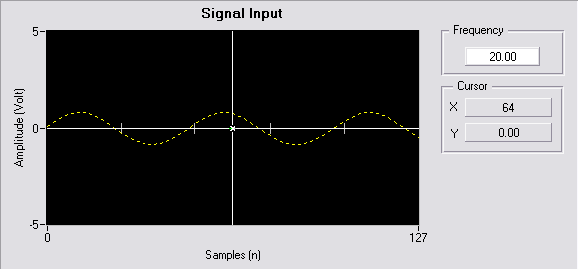
\includegraphics[scale=0.7]{input20hz.png}
\caption{Input sine: $f=20Hz$}
\end{figure}
\begin{figure}[H]
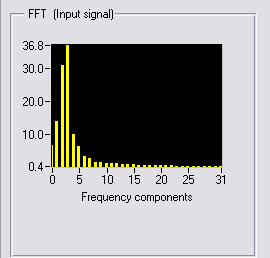
\includegraphics[scale=0.7]{FFT20hz.png}
\caption{FFT: $f=20Hz$}
\end{figure}
\begin{figure}[H]
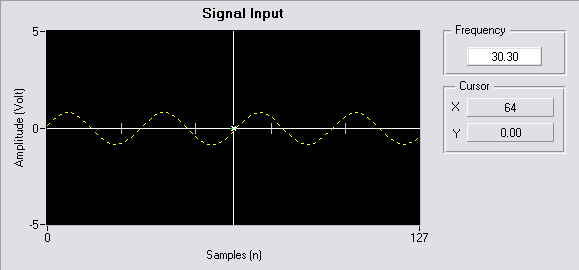
\includegraphics[scale=0.7]{input30hz.png}
\caption{Input sine: $f=30Hz$}
\end{figure}
\begin{figure}[H]
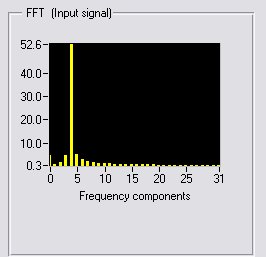
\includegraphics[scale=0.7]{FFT30hz.png}
\caption{FFT: $f=30Hz$}
\end{figure}
\subsection{Opgave 2}
\subsubsection{}
$ \Omega = 2 \pi f T_s = 2 \pi * 20 * \frac{1}{500} = \frac{4\pi}{50}
\Rightarrow N = 25$.
\subsubsection{}
\begin{tabular}{r || l | l | l}
    f & $\Omega$ met $T_s = 0.001$  & Periode $N$ & ?de harm $< \Omega<$ ?de
    harm \\ \hline \hline
    $20 Hz$ & $\frac{4\pi}{50}$ & $25$ & 5de \dots 6de \\ \hline
    $30 Hz$ & $\frac{6\pi}{50}$ & $16\frac{2}{3}$ & 7de \dots 8ste \\ 
\end{tabular}
\subsubsection{}
\begin{figure}[H]
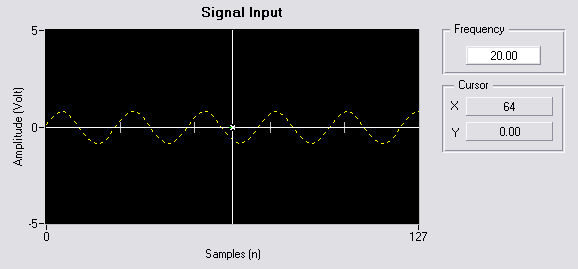
\includegraphics[scale=0.7]{2input20hz.png}
\caption{Input sine: $f=20Hz$}
\end{figure}
\begin{figure}[H]
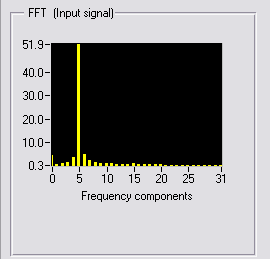
\includegraphics[scale=0.7]{2FFT20hz.png}
\caption{FFT: $f=20Hz$}
\end{figure}
\begin{figure}[H]
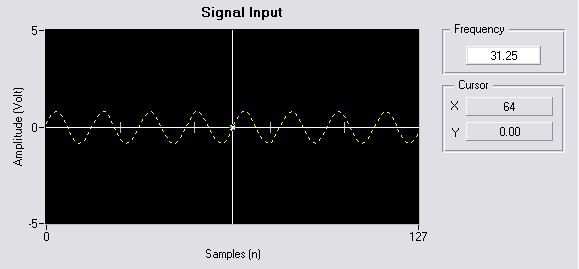
\includegraphics[scale=0.7]{2input30hz.png}
\caption{Input sine: $f=30Hz$}
\end{figure}
\begin{figure}[H]
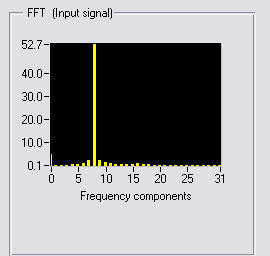
\includegraphics[scale=0.7]{2FFT30hz.png}
\caption{FFT: $f=30Hz$}
\end{figure}
\subsection{Opgave 3}
\subsubsection{}
$ \Omega = 2 \pi f T_s = 2 \pi * 20 * \frac{1}{1000} = \frac{4\pi}{100}
\Rightarrow N = 50$.
\subsubsection{}
$2 * \frac{50\pi}{3200} < \frac{128 \pi}{3200} < 3 *
\frac{50\pi}{3200}\Rightarrow$ The
sine lies between the second and third multiples.
\subsubsection{}
\begin{figure}[H]
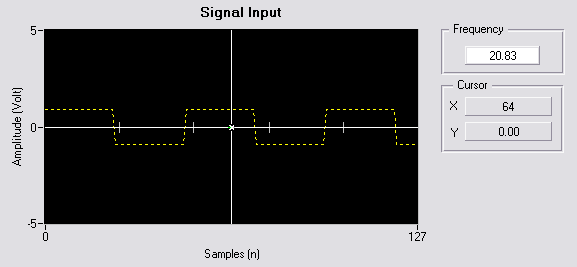
\includegraphics[scale=0.7]{3input.png}
\caption{Input sine: $f=20Hz$}
\end{figure}
\begin{figure}[H]
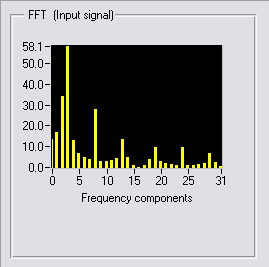
\includegraphics[scale=0.7]{3FFTinput.png}
\caption{Input FFT}
\label{fig:3FFTinput}
\end{figure}
The third, eighth, 13th, 18th, 23rd, 28th, i.e. 3+(5m)th. This is because they
have to be uneven to sum into an approximation of the block-signal.
\subsubsection{}
The transfer function $H(z)$ is defined by $H(z) = K
\frac{z-0}{z-0.9}=\frac{0.5 z}{z-0.9}$
\subsubsection{}
$y[n]-0.9y[n-1]=0.5 x[n] \Leftrightarrow y[n] = 0.9 y[n-1] + 0.5 x[n]$
\subsubsection{}
Maximum amplitude of $\lvert Hz\rvert $ occurs at $z=1$: $\lvert Hz\rvert _{max}
= \frac {0.5}{1-0.9} = 5$. 
\subsubsection{}
In the following figure we see that the maximum frequency contribution after our
low pass filter is around 165, whereas in fig. \ref{fig:3FFTinput} the value was
around 58. 
\begin{figure}[H]
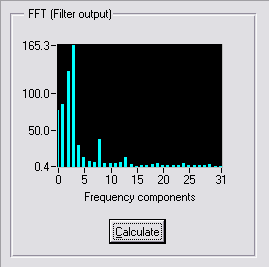
\includegraphics[scale=0.7]{3FFToutput.png}
\caption{Output FFT}
\end{figure}
\subsection{Opgave 4}
\begin{figure}[H]
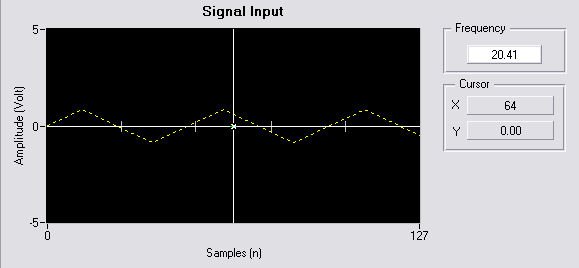
\includegraphics[scale=0.7]{4input.png}
\caption{Output FFT}
\end{figure}
\subsubsection{}
$ \Omega = 2 \pi f T_s = 2 \pi * 20 * \frac{1}{1000} = \frac{4\pi}{100}
\Rightarrow N = 50$.
\subsubsection{}
The strongest neighbouring harmonics are as in Opgave 1, question 2. The ramp
form does not affect this. The following figure confirms this:
\begin{figure}[H]
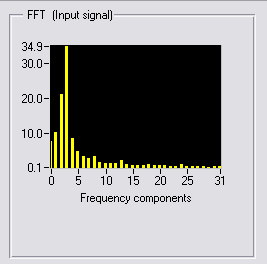
\includegraphics[scale=0.7]{4FFTinput.png}
\caption{Output FFT}
\end{figure}
\subsubsection{}
The strongest harmonics are at the lowest frequencies (harmonics 1 through 4),
with relative peaks at 3, 8, 13 etc. This is similar to the pattern in Opgave 3,
question 3, but with smaller peaks. The smaller peaks can be explained by the
ramp form of the input signal, which requires less of the higher-frequency
harmonic peaks to approximate than the square input signal in Opgave 3.
\subsubsection{}
The second harmonic corresponds to $\frac{4\pi}{128} = \frac{\pi}{32}$, and the
third corresponds to $\frac{6\pi}{128}=\frac{3\pi}{64}$. From this we can derive
$z_1 = \cos{\frac{\pi}{32}}+j \sin{\frac{\pi}{32}}=e^{j\frac{\pi}{32}}$ and 
$z_2 = \cos{\frac{3\pi}{64}}+j \sin{\frac{3\pi}{64}}=e^{j\frac{3\pi}{64}}$.
\subsubsection{}
\begin{figure}[H]
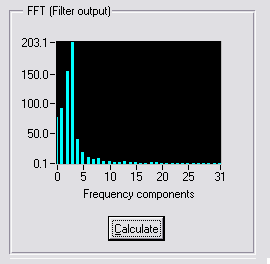
\includegraphics[scale=0.7]{4FFToutput.png}
\caption{Output FFT}
\end{figure}
$H(z)=\frac{z}{z-0.9}$
\subsubsection{}
$\lvert H(z_1)\rvert = \lvert
\frac{e^{j\frac{\pi}{32}}}{e^{j\frac{\pi}{32}}-0.9}\rvert =7.3$ and 
$\lvert H(z_2)\rvert = \lvert
\frac{e^{j\frac{3\pi}{64}}}{e^{j\frac{3\pi}{64}}-0.9}\rvert =5.8$
\subsection{Opgave 5}
\subsubsection{}
$H(z) =
\frac{(z+e^{j\frac{\pi}{10}})(z+e^{-j\frac{\pi}{10}})}{z^2}=
\frac{z^2+e^{j\frac{\pi}{10}}e^{-j\frac{\pi}{10}}-ze^{j\frac{\pi}{10}}-ze^{-j\frac{\pi}{10}}}{z^2}=
\frac{z^2-ze^{j\frac{\pi}{10}}-ze^{-j\frac{\pi}{10}}+1}{z^2}=
\frac{z^2-2z\cos{\frac{\pi}{10}}+1}{z^2}$ \\
$\Rightarrow b_0=1 , b_1 = -2\cos{\frac{pi}{10}} = -1.902113 , b_2= 1 , a_0 = 1,
a_1 = a_2 = 0$ \\
$\Rightarrow y[n] - a_1 y[n-1] - a_2 y[n-2] = b_0 x[n] + b_1 x[n-1] + b_2
x[n-2]$\\
$y[n]= x[n]-2 \cos{\frac{\pi}{10}} x[n-1] + x[n-2]$.
\subsubsection{}

\begin{tabular}{r || l | l}
    f & $\Omega$ with $T_s = 0.001$ & $\lvert H (e^{j\Omega})\rvert$ \\ \hline \hline
    $10Hz$  & $2\pi \times 10 \times 0.001 = \frac{\pi}{50}$ & $\lvert
    H(e^{j\frac{\pi}{50}})\rvert = 0.093941$ \\ \hline
    $20Hz$  & $\frac{4\pi}{100} = \frac{\pi}{25}$ & $0.082116$ \\ \hline
    $30Hz$  & $\frac{6\pi}{100} = \frac{3\pi}{50}$ & $0.062462$ \\ \hline
    $40Hz$  & $\frac{8\pi}{100} = \frac{2\pi}{25}$ & $0.03505$ \\ \hline
    $50Hz$  & $\frac{10\pi}{100} = \frac{\pi}{10}$ & $0$ \\ \hline
    $60Hz$  & $\frac{12\pi}{100} = \frac{6\pi}{50}$ & $0.04256$ \\ \hline
\end{tabular}\\
$\Omega 2\pi \times f \times T_s = 2\pi \times 10 \times \frac{1}{1000} =
\frac{20\pi}{1000}=\frac{2\pi}{100}$\\
$\Omega 2\pi \times 20 \times T_s = 2\pi \times 20 \times \frac{1}{1000} =
\frac{40\pi}{1000}=\frac{4\pi}{100}$\\
$\Omega 2\pi \times 30 \times T_s = 2\pi \times 10 \times \frac{1}{1000} =
\frac{60\pi}{1000}=\frac{6\pi}{100}$\\
$\lvert H(z) \rvert = \frac{z^2 - 1.90211321}{z^2} =
\frac
{
(e^{j\frac{\pi}{50}})^2 
-1.902113 \times e^{j\frac{\pi}{50}}+1
}
{
(e^{j\frac{\pi}{50}})^2
}$
\subsubsection{}
Our experiment confirmed that the $50Hz$ frequency was filtered out, as derived
and listed in the table above. We can conclude that the filter we have created
is a band-stop filter that attenuates frequencies in the region of $50Hz$.
\end{document}
